%!TEX root = twig-gpu.tex

\section{Method Overview}

In Twig, we write \emph{rules} which express some high-level operation, such as kernel execution or copying data to a device, as a function on \emph{types}. A Twig program is evaluated with a type given as input. The output is another type, transformed by the combined rules of the program. As a side-effect, C code is generated which performs the transformation on values in C. This basic idea is formalized in Sec.~\ref{sec:semantics}.

Types in Twig are based on the set provided by C, but may be augmented with additional information. For GPU programming, we augment standard data types with a \emph{location}. The location information describes where the data is stored in memory; in this case, either in the main system memory or on the GPU. For example, we can represent an array of \texttt{int}s on the CPU with the Twig type \texttt{array(int)}. The same type located on the GPU is \texttt{gpu(array(int))}. Any standard type may be wrapped inside the \texttt{gpu} type constructor.

Note that location information is only used by Twig during evaluation and code generation. In particular, it may not be reflected in the types for the generated code. If we are generating CUDA code, for example, the generated type for both \texttt{gpu(array(int))} and \texttt{array(int)} is simply a C pointer to \texttt{int} (i.e., \texttt{int *}). In this case, the location information is erased during the code generation phase. For other target languages or APIs that have a notion of location, the information could be preserved in the target data types.

By augmenting basic data types with location information, we ensure that rules must be specific to the GPU in order to operate on GPU data. For example, a rule

\begin{verbatim}
[gpu(array(float)) -> gpu(array(int))]
\end{verbatim}

converts an ``array of floats'' data type to an ``array of integers'' type if and only if the type describes data located on the GPU. If the type describes data located elsewhere, its type must be ``converted'' (i.e., the data copied to the device) with a rule such as

\begin{verbatim}
[array(float) -> gpu(array(float))]
\end{verbatim}

This simple scheme enables Twig to reason about requirements for data motion.

It is important to understand that rules such as those given above describe transformations on \emph{data types}, not on the data themselves. It falls to the code that is generated as a consequence of successful application of these rules to perform the promised conversion on the actual data. Code generation is described in Sec.~\ref{sec:code-gen}.

Our scheme could be extended to support multiple GPU devices, with each device corresponding to a unique located type. In fact, we think that located types could be useful in a variety of situations; this is a topic of ongoing work.

% TODO: This needs to be moved somewhere else.
\subsection{Redundant Data Movement}

We illustrate the redundant data movement problem in Fig.~\ref{fig:redundant-movement}. In the diagram, two GPU kernel transformations, $f$ and $g$, are called in sequence. The na\"ive composition is shown in Fig.~\ref{fig:redundant-movement}(a). This case has redundant data movement. The arrangement in Fig.~\ref{fig:redundant-movement}(b) is the desired composition, with the redundant intermediate copying operations eliminated.

\begin{figure}[ht]
\centering
\begin{tabular}{cc}
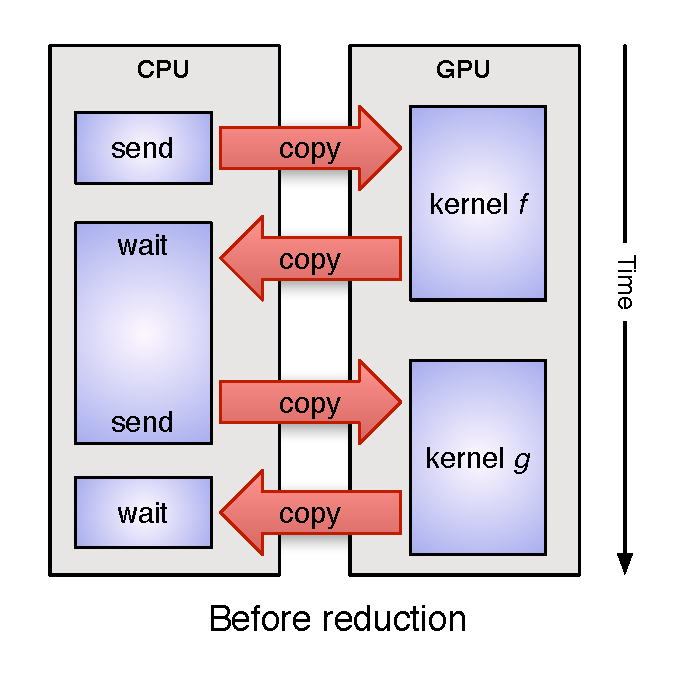
\includegraphics[width=2in]{images/reduction-before}&
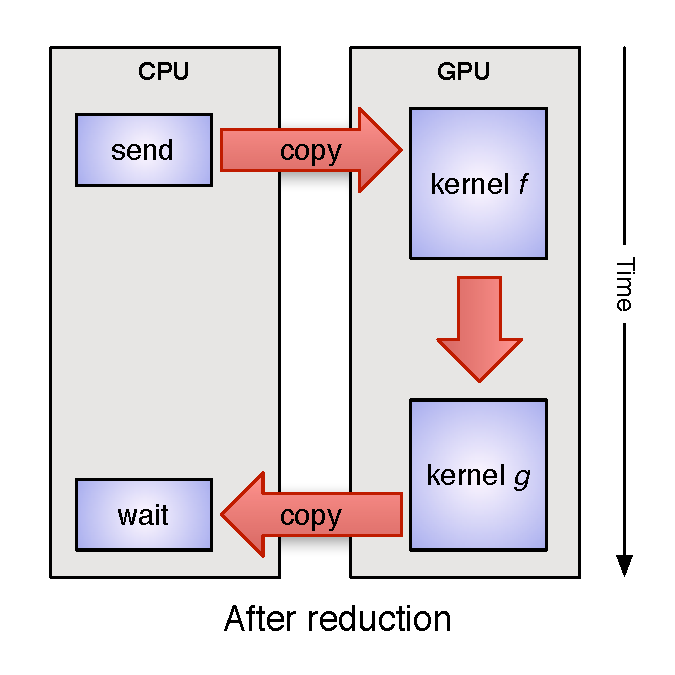
\includegraphics[width=2in]{images/reduction-after}\\
(a)&(b)\\
\end{tabular}
\caption{Elimination of redundant data movement. Part (a) depicts two GPU kernels called in sequence, unnecessarily copying data to and from the device. Part (b) shows the same program with the redundant copies removed.}
\label{fig:redundant-movement}
\end{figure}
